\section{blockchian stuff} % change title

\cite{baran_distributed_1964} introduced distributed networks, using a new concept in which computers are connected to other stations rather than switching points like in a centralised system.

Distributed systems are defined as a system in which hardhware or software components located at networked computers communicatte and coordinate their actions via message passing. \cite{coulouris_distributed_2011}

As stated in \cite{coulouris_distributed_2011}, a distributed system must accommodate heterogeneous hardware, operating systems and networks. The networks may differ widely in performance. Systems of widely differing scales, ranging from tens of computers to millions of computers, must be supported.

Replication is key to the effectiveness of distributed systems, it can provide enhanced performance, fault tolerance and high availability. \cite{coulouris_distributed_2011}

nodes in distributed systems can be honest, faulty or mailcious. \cite{bashir_mastering_2017}
\cite{coulouris_distributed_2011} defines arbitrary failures as follows. The term arbitrary or Byzantine failure is used to describe the worst possible failure semantics, in which any type of error may occur. 
For example, a process may set wrong values in its data items, or it may return a wrong value in response to an invocation.

In \cite{lamport_byzantine_1982} the thought experiment of The Byzantine Generals Problem was proposed. 
The scenerio depicts a group of army generals, leading different parts of the Byzantine army plan to attack or retreat from a city. 
The generals can only communicate with eachother via messenger. Communication is necessary in agreeing on a strategy to avoid failure. 
The problem being that one or more of the generals may be traitorous and is attempting to prevent the others from reaching an agreement. 
This necessitates a viable mechanism that enables agreement between actors in the presence of traitors. 
Analogously, distributed systems require agreement amongst nodes, whilst using a channel for communication, even in the presence of Byzantine nodes. This is known as the consensus problem. \cite{fischer_consensus_1983}
The consensus problem occurs when attempting to achieve reliability in a distributed system, in the presence of faulty processes. 
A system requires processes to reach an \emph agreement on a value after one or more processes propose what the value should be. 
In a system such that: each process $p_i$ communicates with other processes via message passing (assuming communication is reliable), up to some number $f$ of the $N$ processes are faulty, the remainder of processes are correct.\linebreak[1]
Reaching consensus is achieved as follows. 
Every process $ p_i $ starts in an \emph{undecided} state and \emph{proposes} a single value $v_i$.
The processes communicate with eachother and exchange values. 
Each process then sets the value of a \emph{decision variable}, $d_i$. 
In doing so the process enters the \emph{decided} state and can no longer change $d_i$.\cite{coulouris_distributed_2011}
\begin{enumerate}
	\item Termination: Eventually each correct process sets a decision variable.
	\item Agreement: The decision of all correct processes is the same.
	\item Integrity: If the correct processes al proposed the same value, then any correct process in the \emph{decided} state has chosen that value.\cite{coulouris_distributed_2011}
\end{enumerate}

The Byzantine Generals Problem was solved in \cite{castro_practical_1999}, where the Practical Byzantine Fault Tolerance (PBFT) algorithm was introduced.

The first practical implementation of PBFT was produced with the inception of Bitcoin, in which the Proof-of-Work (PoW) algorithm was developed as a consensus mechanism. \cite{nakamoto_bitcoin_2019}

In \cite{ongaro_search_2014}, Raft was introduced as a consensus algorithm, which produced similar results to and was as efficient as Paxos - a family of protocols for solving consensus, presented in \cite{pease_reaching_1980}.
Raft was a successful attempt at restructuring a consensus mechanism in order to enhance understandability. Raft is crash fault tolerant, but lacks in Byzantine fault tolerance. \cite{ongaro_search_2014} 


Ledger is the sequenced, tamper-proof ... 

chain is transaction log, structured as hash-linked blocks where each block contains a sequence of $N$ transactions.

Rethinking Permissioned Blockchains \cite{vukolic_rethinking_2017} 

\subsection{Healthcare Stuff} % change heading


use these: 

\cite{paranjape_implementation_2019} $ <-- $ Implementation Considerations for Blockchain in Healthcare Institutions

\cite{yu_comparison_2020} $<--$ 'Comparison of Smart Contract Blockchains for Healthcare Applications'

\cite{stamatellis_privacy-preserving_2020} $<--$ 'A-Privacy-Preserving-Healthcare-Framework-Using-Hyperledger-Fabric'

\subsubsection{FHIR}
FHIR - standards for sharing healthcare information.\linebreak[1]

\subsection{Security}

a reference = \cite{brotsis_security_2020} $<--$ 'On the Security and Privacy of Hyperledger Fabric - Challenges and Open Issues'

Whilst penetration testing Hyperledger Fabric, there was found a high severity issue, which describes the potential to guess the content of a Private Data Collection.
This is achieved using SHA256 as an oracle. To ensure this vulnerability is not available in the system, it is necessary to ensure any private data is salted before being hashed. \cite{shaw_penetration_2019}

\section{benefits}
[Covid-19: Vaccines and vaccine passports being sold on darknet] - this system would negate these spoofed vaccination records as all data will be on the system and if not it's illegitimate.
\linebreak[3]

\section{System Design}

Usage of Raft or Kafka is sufficient as Byzantine fault tolerance is not required in the proposed sysetem, as the nodes shall be controlled by trusted authorities.
Though, a Byzantine fault-tolerant ordering service for Hyperledger Fabric has been developed, this would be useful if nodes were prone to malicious activity. \cite{sousa_byzantine_2018}

\cite{yusuf1_comparison_2020} states that Raft is superior to Kafka in terms of success and speed when conducting invoke transactions due to its simpller framework. But, when querying transactions Kafka is superior since the throughput rate is larger.
So, which one ??

Developing and testing chaincode was initially performed using the Fabric test network, provided in the official documentation for Hyperledger Fabric \cite{noauthor_using_nodate}, contained in the "fabric-samples" repository \ref{appendix:testnet}.
It is based on a limited configuration:
\begin{enumerate}
\item{It includes two peer organizations and an ordering organization.}
\item{For simplicity, a single node Raft ordering service is configured.}
\item{To reduce complexity, a TLS Certificate Authority (CA) is not deployed. All certificates are issued by the root CAs.}
\item{The sample network deploys a Fabric network with Docker Compose. Because the nodes are isolated within a Docker Compose network, the test network is not configured to connect to other running Fabric nodes.} \cite{noauthor_using_nodate}
\end{enumerate}


Currently, medical data has the HL7 standard as a data exchange format but the
exchange of medical records between countries is not widespread. \cite{kung_personal_2020}

\subsection{Default application SDK}
Go is best for chaincode but what would be the most suitable for the access applications? Java, because it's already highly used in enteprise already? **find reference for this ** 
Java also enables cross-platform usage, most convenient for these systems that are already up and running. - Node satisfies these conditions also, Node has Performance Traffic Engine in fabric-test toolset.
Fabric Network Operator tool, from Hyperledger, also utillises the Node SDK, looking like the project might just wanna use Node? Benefits to web app vs desktop? 
Java is probs more secure ** find ref ** but web app with Node would likely be more flexible, as it can be used for the access application as any device runs Node but internet is required.
Java is statically typed, but this is also achieved when using TypeScript with Node - this brings both SDKs to an equal playing field, in terms of maintainability.
Orgs will be able to develop their own applications, enabled by OSS. However, considerations are in place for the best default SDK to use, as the correct choice could simplify adoption.

Does Node possess an advantage in terms of ease of adoption? Can more mobile devices use Node than Java? Does it even matter which SDK? 


\subsection{Hyperledger Fabric}
Hyperledger fabric is ... Using their MSPs is different to things like this \url{'https://www.hyperledger.org/blog/2020/04/21/trustid-a-new-approach-to-fabric-user-identity-management'}{TrustID: A New Approach to Fabric User Identity Management} how? Why are we not customising and instead going with fabric's defaut implementation, maybe because it fits our use case better? It makes sense as the orginisations using the system are governed already by their heath body, for UK it's MAYBE Department of Health \& Social Care - look this up! See if there's a general term for lead health body or whatever

Fabric has all the identity functionality built in, Indy + Aries would be more flexible but does that matter with an permissioned network? Fabric MSPs etc vs DIDs? Or does it use DIDs? \url{'https://www.w3.org/TR/did-core/'}{w3 DIDs}


Transaction flow "The SDK serves as a shim to package the transaction proposal into the properly architected format (protocol buffer over gRPC) and takes the user’s cryptographic credentials to produce a unique signature for this transaction proposal." - \url{"https://hyperledger-fabric.readthedocs.io/en/latest/txflow.html'}.\linebreak[1]


Enforcing Determinism of Java Smart Contracts \cite{spoto_enforcing_2020}

\url{'https://wiki.hyperledger.org/display/fabric/Design+Documents'} WRITE ABOUT THIS!

Ensuring determinism in smart contracts is essential % why? ref?

This first phase also eliminates any non-determinism, as inconsistent results can be filtered out before ordering.
Because we have eliminated non-determinism, Fabric is the first blockchain technology that enables use of standard programming languages. \cite{androulaki_hyperledger_2018}

\subsubsection{Architecture Overview}

Hyperledger Fabric's key design features, as introduced in \cite{androulaki_hyperledger_2018}, are explored in the following text.
Asset, defined by chaincode, are exchanged across the network. These can range frmo the tangible to teh intangible. These are stored as a collection of key-value pairs, represented in binary and/or JSON, with state changes recorded as transaction on a channel ledger. 
Chaincode, the software defining assets, also defines the transaction instructions for manipulating the assets; chaincode is the business logic. Invocation of chaincode is recorded in the ledger.
The ledger is described in \cite{noauthor_hyperledger_nodate} as the "sequenced, tamper-resistant record of all state transitions in the fabric." This ledger is comprised of a blockchian to store the records in blocks and a state database. 
Channels are used to communicate privately between organisations, enabling privacy.
Each channel contains a ledger, for that channel, peers also maintain a copy of the ledger for each channel of which they participate. This is used to maintain consistency across peers. 


Hyperledger projects follow a design philosophy, which includes a modular, extinsible approach; enabling interoperability.
Design puts an emphasis on secure solutions, crucial to systems using sensitive data.
Hyperledger's token-agnostic approach simplifies bringing blockchain to business infrastructure. \cite{noauthor_hyperledger_2017}

Hyperledger projects embrace security by design and follow the best practices specified by the Linux Foundation's Core Infrastructure initiative. \url{https://www.coreinfrastructure.org/}

As discussed in \cite{androulaki_hyperledger_2018}, blockchain systems typically, both permissioned and permissionless, follow the order-execute architecture. 
This execution style involves ordering transactions first, using a consensus protocol, then executes them in the same order on all peers sequentially.\footnote{This report follows the convention set in the Hyperledger Fabric whitepaper of calling the transaction execution (named "transaction validation" in blockchains such as Bitcoin) \emph{transaction execution} to bring the terminology together.}
\begin{figure}[H]
  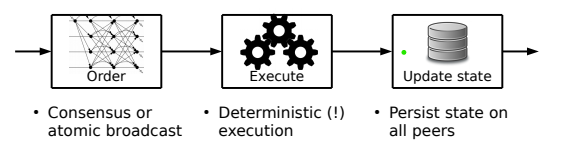
\includegraphics[scale=0.9]{order-execute}
  \caption{Order-execute architecture in replicated services}
  \source{\cite{androulaki_hyperledger_2018}}
\end{figure}

Whilst the order-execute architecture is conceptually simple and therefore widely used, there are drawbacks which occur when using it for a general-purpose permissioned blockchain.\cite{androulaki_hyperledger_2018}
The most significant disadvantages are as follows: 
\emph{Sequential execution}. Executing transactions sequentially on all peers limits the effective throughput that can be achieved on the blockchain.\cite{androulaki_hyperledger_2018} 
One solution to this problem, used by Ethereum \cite{wood_ethereum_nodate}, utilises the concept of \emph{gas} consumed by a transaction execution, which is converted at a \emph{gas price} to a cost in the cryptocurrency and billed to the transaction submitter.
This solution is excellent for use in permissionless blockchains, though does not suffice when designing a general-purpose, permissioned, token-agnostic, blockchain like Hyperledger Fabric. \cite{androulaki_hyperledger_2018} \linebreak[1]

% ADD ABOUT FABRIC MODEL AND FIGURE OF IT'S EXECUTION STYLE

Hyperledger Fabric distributed applications consist of two parts: A smart contract, called \emph{chaincode}, which is program code that implements the application logic and runs during the \emph{execution phase}.
As well as an \emph{endorsment policy} that is evaluated in the \emph{validation phase}. \cite{androulaki_hyperledger_2018} \linebreak[1]

This system is utilising v2.2, the LTS release of the second major release of Fabric. 
Fabric v2.0 delivers important new features and changes for users and operators. % Support for new application and privacy patterns, enhanced governance around smart contracts, and new options for operating nodes. 
Namely, the addition of decentralised governance for smart contracts. 
A new implementation of the chaincode lifecycle allows multiple organisations to agree on parameters of chaincode, before it can be used to interact with the ledger. 
These parameters could be ... % finish 
\cite{noauthor_whats_nodate}

In Fabric, to participate, every node and user that interacts with a network needs to be part of an organisation. \cite{noauthor_using_nodate}

Members of a network in Fabric enroll through a trusted Membership Service Provider (MSP). \cite{noauthor_introduction_nodate}
An MSP serves as a trusted authority, that is in control of the governing of identities for its organisation. 

An MSP is a structure of folders added to the network configuration, to define the permissions and roles in an organisation. 
Certificate Authorities generate the certificates that represent identities, the MSP is where these reside. 
Roles in organisations are assigned to the identities, by the MSP. 
MSPs also hold a copy of the revoked certificates, for the organisation, which is checked whenever the certificate is attempting to be used. \cite{noauthor_membership_nodate}
This list is called a Certificate Revocation List (CRL) \cite{cooper_internet_nodate} and is stored by the issuing CA. \cite{noauthor_identity_nodate}
MSPs come in two flavors, \emph{local MSPs} have a scope limited to the organisation they are part of and reside on the organisation's node. Every node requires an MSP.
\emph{Channel MSPs} define administrative and participatory rights at a channel level. These channel MSPs include the MSPs of the organisations on the channel, enabling the control of relationships between the channel participants. \cite{noauthor_membership_nodate}

Fabric CA is the default Certificate Authority in a Fabric network. Acting as a root CA, Fabric CA issues the certificatse required for the MSPs to implementend identities and roles. \cite{noauthor_identity_nodate}


\subsubsection{Privacy by Design}

\cite{noauthor_private_nodate} $<--$ private data collections, is privacy by design - enables GDPR compliancy etc = \cite{narumanchi_privacy_2019} $<--$ Privacy by Design Helps Blockchains Comply With GDPR

%  Hyperledger Fabric offers privacy protection in the way of four aspects. Firstly, asymmetric cryptography and zero-knowledge proof separate the transaction data from on-chain records, protecting privacy from the underlying algorithm. Secondly, the digital certificate management service guarantees the legitimacy of the organization on the blockchain. Thirdly, the design of multi-channel separates the information between different channels. Finally, privacy data collection further satisfies the need for the isolation of privacy data between different organizations within the same channel. In the above measures, the two most distinctive methods are the channel and privacy data collection
Hyperledger Fabric has an excellent offering of privacy protection features.
Asymmetric cryptography and zero-knowledge proof separate the transaction data from records on chain. 
Identities for network actors are encapsulated in X.509 digital certificates and are controled by MSPs as aforementioned. \cite{noauthor_identity_nodate}. 
A X.509 digital certificate or public key certificate is a signed document which holds information on the identity to which the certificate has been issued, as well as the identity that issued it known as a Certificate Authority (CA). 
These certificates are based on the widely accepted X.509 Public Key Infrastructure (PKI). \cite{cooper_internet_nodate}
Fabric utilises certificate chains, a concept defined using the name \emph{certification path} in \cite{cooper_internet_nodate}, which Hyperledger calls a \emph{Chain of trust}, to distribute the responsibiity of issuing certificates. 
The processes uses \emph{Intermediate CAs} which have their certificates issued by a Root CA. 
This allows for backtracking to find the Root CA of any issued certificate, this helps scaling remain secure and limits the exposure of Root CAs - which if compromised would endanger the \emph{Chain of trust}. \cite{noauthor_identity_nodate}
The \emph{Chain of trust} is depicted in \ref{fig:trustchain}.
\begin{figure}[H]
  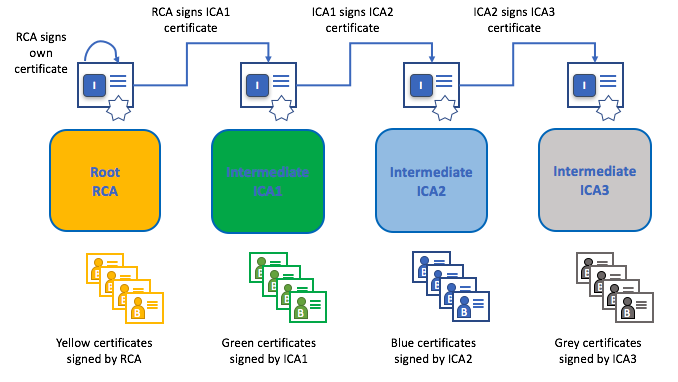
\includegraphics[scale=0.6]{identity-diagram}
  \caption{CA chain of trust in Fabric}
  \source{\cite{noauthor_identity_nodate}}
  \label{fig:trustchain}
\end{figure}

% explain cryptogen, configtxgen, configtxlator? check which ones we actually use lol cause I think I remember maybe some of these being only for test-network???


\cite{ma_privacy_2019} $<--$ The privacy protection mechanism of Hyperledger Fabric and its application in supply chain finance





\subsubsection{Inspiration} %- from hyperledger fabric projects, redo title
Use $-->$ \cite{yuan_design_2018}. <-- says there is a "LACK OF UNIVERSALLY DEFINED STANDARDS" is this true still? should this report be proposing standards for blockchain healthcare systems, are there thusfar?

\subsubsection{Consensus}

In Hyperledger business blockchain frameworks consensus is reached by performing two seperate activities:
\begin{enumerate}
  \item Ordering of transactions
  \item Validating transactions
\end{enumerate}
In the first step, the transactions are received from the client.
An ordering service is used to order the transactions. 
To enable confidentiality, the ordering service may be agnostic to the transaction; that is, the transaction content can be hashed or encrypted.\cite{noauthor_hyperledger_2017}
This is extremely benificial to this system, as maintaining confidentiality is essential to abiding by the GDPR \cite{noauthor_general_nodate}.

Consensus in Hyperledger Fabric is further broken into 3 phases: \emph{Endorsement}, \emph{Ordering} and \emph{Validation}.
\begin{enumerate}
  \item Endorsement is driven by policy (eg. m of n signatures) upon which participants endorse a transaction. 
  \item Ordering phase accepts the endorsed transactions and agrees to the order to be committed to teh ledger.
  \item Validation takes a block of ordered transactions and validates the correctness of the results, including checking endorsement policy and double-spending.
\end{enumerate}
zero-knowledge asset transfer vs zero-knowledge proof? \linebreak[1]
Using Go chaincode, generating UML diagrams from this, classes such as: Record, with states: immunised or not?

\section{System Architecture Overview}

going to call the "admissions staff" (people who want to check immunisation information) Verifiers.

Each organisation in the network has control over its members, through Fabric's MSPs. 
This control also extends to the organisation's data, this shall not be shared with other organisations unless allowed by the organisation. 
Private channel capabilities ensure that data will only be shared with those authorised by the owning organisation. 

Fabric's test-network was used in the initial design of the network for the DIIS \ref{appendix:testnet}. The test network, as described previously, enables the testing of chaincode and applications without setting up a dedicated network. 
This is excellent for the development process. 

\section{}

\section{Chaincode}

\cite{alexaki_blockchain-based_2018} suggests that medical records should contain metadata of a patient-provider encounter (visit date/time, location, etc.), 
the data stored off-chain and should be entered when the record is produced. As immunisations expire, the ledger must store metadata on immunisations to ensure the record in the ledger can be invalidated when the date is reached.

Chaincode is Hyperlegder Fabric's version of smart contracts. Chaincode is a program, which can be written in general-programming languages Go, JavaScript (for Nodejs runtime) or Java, that implements a prescribed interface.

Selected Go, as there are apparent benifits outlined in \cite{foschini_hyperledger_2020}

The duration of protection conferred by vaccines should
be tied to passport expiry dates \cite{dye_covid-19_2021}.
This is implemented via the expiration of our Record contract.

The chaincode for this system will represent "Records", immunisation records, the initial chaincode package will be called "record\_1.0". The implementation of this is documented below. 
Representing the records as chaincode, or smart contracts, enables the manipulation of records by organisations that "own" them. The "Owner" shall be recorded inside the Record contract. 
The chaincode written for this system can be found at \ref{appendix:chaincode}.

\subsection{Implementation}
Fabric networks use chaincode to initialise and manage the ledger state, through transactions submitted by applications. \cite{noauthor_writing_nodate}
To use chaincode in a network organisations need to agree to the parameters, the name of the chaincode, version and the endorsement policy. 
\cite{noauthor_writing_nodate} explains that the agreement is reached using the following steps:
\begin{enumerate}
  \item Package the Chaincode
  \item Install the chaincode on peers: Each organisation that will utilise the specific chaincode, to endorse transactions or query ledgers, needs to execute this step.
  \item Approve chaincode definition for organisation: This step also requires completion from each organisation that will use the chaincode. By default, the chaincode needs to be approved by atleast a majority of organisations before it can be deployed on a channel.
  \item Commit the chaincode definition to the channel: After the chaincode is approved by a sufficient number of organisations, one organisation can commit the chaincode definition.
\end{enumerate}

Chaincode needs to be packaged in a tar file for it to be installed onto peers \cite{noauthor_fabric_nodate}. Using the Fabric peer binaries, the following command can be used to skip manually adding the necessary "metadata.json" file which required in the tar file.
\begin{lstlisting}[language=bash, caption={peer lifecycle chaincode package command}]
  # create the chaincode package using the peer lifecycle chaincode package command
  peer lifecycle chaincode package record.tar.gz --path ../asset-transfer-basic/chaincode-go/ --lang golang --label record_1.0
\end{lstlisting}

Though not necessary for Fabric networks, it would be useful for organisations to synchronise their labels for chaincode. This will be a standard for adopting this system.

Installation of chaincode on peers can be executed via CLI or an SDK \cite{noauthor_fabric_nodate}. % come back and talk about if we added SDK / just say you need to use CLI for this DIIS network.

\begin{figure}[H]
  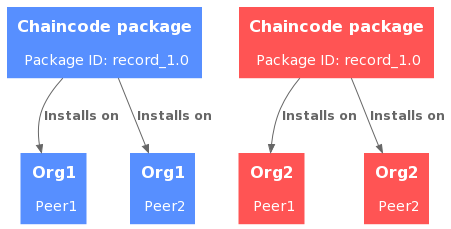
\includegraphics[scale=0.7]{cc-diagram-redo}
  \caption{Peer admin from two organisations installs the chaincode package record\_1.0}
  \source{Adapted from \cite{noauthor_fabric_nodate}}
\end{figure}

In this system is it not necessary to set the endorsement policy for the chaincode as it will be utlising the default value, which requires that a majority of organisations endorse a transaction. \cite{noauthor_fabric_nodate}

\section{Immunisation Verification}
smarthealth.cards by Vaccination Credential Initiative (VCI) - smart card framework.\linebreak[1]

Use an SDK to invoke chaincode that compares the provided data (hash of the transaction? - in which your immunisation record is stored) with the hash (SHA-250 probs) of the data in the ledger. If there's no match there's no verification, details?

\section{Blockchian-as-a-Service}

Using Blockchain for Electronic Health Records \url{'https://ieeexplore.ieee.org/stamp/stamp.jsp?tp=&arnumber=8863359'} \cite{shahnaz_using_2019} 


**shortcomings are discussed here: \url{'https://ieeexplore.ieee.org/document/9284197'} \cite{brotsis_security_2020} ** . The computing power and security provided by BaaS can make up for the shortcomings aforementioned.\cite{song_research_2021}.

Comparing Blockchain-as-a-Service platforms, to identify which tool is most suitable for delpoying the proposed Distributed Immunisation Information System built with Hyperledger Fabric.\linebreak[1]

Reading \cite{onik_performance_2019}.\linebreak[1]

[Performance Analytical Comparison of Blockchain-as-a-Service (BaaS) Platforms] says "Blockchain highly suffers from scalability problem due to its capped transaction
latency as well as consensus approach"\linebreak[1]

Azure have FHIR API, is it the only one? looks like maybe Amazon also \url{'https://azure.microsoft.com/en-gb/services/azure-api-for-fhir/?ocid=AID754288&wt.mc_id=azfr-c9-scottha%2CCFID0475'}{Azure FHIR API}
\linebreak[1]

Beginning, I was aware of two options: Azure and IBM.\linebreak[1]

\subsection{IBM Blockchain Platform}
To ensure all organisations can setup the necessary infrastructure, it's most simple to use a Blockchain-as-a-Service platform. 
IBM Blockchain Platform for IBM Cloud is built with Hyperledger Fabric v1.4.11 and v2.2.2. The system proposed in this report uses v2.2.2, as it delivers delivers important new features and changes for users and operators alike, including support for new application and privacy patterns, enhanced governance around smart contracts, and new options for operating nodes. \cite{noauthor_whats_nodate}

useful for tesing, this uses This code pattern uses IBM Db2 federation capabilities to perform SQL analytics on a sample blockchain insurance application using Hyperledger Fabric. 
This code pattern uses the sample blockchain insurance application. Apache Zeppelin notebook will be used to perform analytics by querying the blockchain using Db2 and SQL. - https://developer.ibm.com/patterns/use-db2-and-sql-to-perform-analytics-on-blockchain-transactions/

May have to use IBM just because of their whole hybrid cloud infrastructure, could be too easy to give up \cite{noauthor_ibm_2020}
\linebreak[1]
Requested demo of IBM Health Pass, will look more into this physically when the change occurs. For now, review the literature provided publicly - not much lmao \url{'https://www.ibm.com/watson/health/resources/digital-health-pass-blockchain-explained/'}
\url{'https://mytechdecisions.com/compliance/ibm-salesforce-work-covid-19/'}
